% !TEX encoding = UTF-8 Unicode
%!TEX root = ../Main/thesis.tex
% !TEX spellcheck = en-US
%%=========================================
\documentclass[../Main/thesis.tex]{subfiles}
\begin{document}
\chapter{Development}\label{ch:development}

\section{Requirements}%
\label{sec:requirements}
To establish requirements for the subsequent re-implementation of the
``visualizer'' component we will take a look at the current implementation, and
how the system works. The overarching requirements is the development and the
resulting project being a contribution to the Open-Source community.

\section{Rebuilder}\label{sec:development_rebuilders}
The purpose of the rebuilder is to watch for new packages, queue them, build the
package in a clean environment to reproduce the package, and then publish this
result so we can query them later when installing packages.

To achieve this we need to fulfill a few requirements:

\begin{enumerate}
    \item \label{itm:published} We need to know when a package is published.
    \item \label{itm:scheduler} Something needs to schedule the new packages.
    \item \label{itm:builder} We need to build the package in a clean environment.
    \item \label{itm:publish} We need to publish results of the built package.
    \item \label{itm:transport} We need to check the results when installing packages.
\end{enumerate}

It is important to remember that this system is only targeted Debian as
supporting is universally would require a lot of engineering effort and handling
of special cases.

\begin{figure}[H]
  \centering
  \begin{sequencediagram}
    \newthread{buildinfo}{buildinfo server}{}
    \newthread{scheduler}{scheduler}{}
    \newthread{redis}{redis}{}
    \newthread{builder}{builder}{}
    \newthread{visualizer}{visualizer}{}
    \begin{call}{scheduler}{NewBuildinfo()}{buildinfo}{}\end{call}

    \begin{call}{scheduler}{rpush}{redis}{}
        \postlevel
    \end{call}

    \prelevel\prelevel
    \setthreadbias{east}

    \begin{call}{builder}{rpop}{redis}{}
        \postlevel
    \end{call}

    \setthreadbias{center}
    \begin{callself}{builder}{build}{}
    \end{callself}
    \begin{messcall}{builder}{publish}{visualizer}{}\end{messcall}
  \end{sequencediagram}
\caption{rebuilder sequence diagram}
\label{lst:rebuilder_sequence_diagram}
\end{figure}

The overlying architecture is displayed in~\ref{lst:rebuilder_sequence_diagram} as
a sequence diagram. It gives a quick overview how the different parts interact
with each other in sequence for one successful package rebuild.


\subsection{buildinfo.debian.net}%
\label{sub:buildinfo_debian_net}
The goal is to rebuild packages released by Debian, but getting this information
directly for a Debian package mirror can be tedious. What we instead do is
relaying on the buildinfo server created by the Debian project to keep track of
all published buildinfo files from built packages. This gives us a canonical
view of all packages built by Debian infrastructure.

% TODO: Add refference to pull request
To utilize this service we need to keep a track of all newly submitted files,
however the current API does not support this. To get around this we submitted a
code change so we would be able to get all files submitted after a given
timestamp. As of writing this code change is not accepted.

The rebuilder system has instead relied on a copy of the server with the code
change included so we are able to monitor new buildinfo files.

\subsection{scheduler}%
\label{sub:scheduler}
The scheduler is a small service which monitors the endpoint and schedules any
new files found from the buildinfo server. Currently it pushes new package files
to redis, which is a very simple key value store, to help schedule the builders.
This enables us to add an arbitrary number of builders. This is important for a
few reasons. It helps scaling the system if its needed, and it also allows to
have builders with different architectures to build packages.

Because of builder constraints the current scheduler does not add builds on
other architectures then ``amd64''.

\subsection{builder}%
\label{sub:builder}
The builder consists of a service that queries redis after new items on a timer.
When new builds are dispatched, the build is done by utilizing the buildinfo
files as provided by the Debian build server. The build are done with the tool
``srebuild''.

``srebuild'' is a Perl script used to build packages in a clean environment.
With this environment the buildinfo is parsed and all missing dependencies are
acquired to recreate the package. The source packages, which contains the source
and the build files needed to build the package, is acquired from a mirror and
the build is done. When the build is done, the results are signed with a
cryptographic key, to verify that the build server did produce the files, and
then published to the visualizer.


\subsection{visualizer}%
\label{sub:visualizer}
The visualizer is the component which displays the rebuilt packages in a web UI.
The user is also able to fetch the buildinfo and linkmetadata files. The current
implementation is a short snippet of code backed by a sqlite database to aid in
displaying the needed webpages. The implemented API as seen in
\ref{api:old_visualizer} is simplistic and provides the needed features to let
users verify builds.


\begin{table}[H]
\footnotesize
\centering
\settowidth\tymin{\textbf{Endpoint}}
\setlength\extrarowheight{2pt}
\begin{tabulary}{\textwidth}{|l|L|l|L|}
\hline
    \textbf{Endpoint} & 
    \textbf{Type} & 
    \textbf{Parameters} & 
    \textbf{Description} \\
\hline
    /new\_build & POST$^1$ & metadata, buildinfo & Submit a new build \\  \hline
    /sources/<name> & GET & & Gets the available builds for a package \\  \hline
    /sources/<name>/<version>/buildinfo& GET & & Gets the BUILDINFO file for a build \\  \hline
    /sources/<name>/<version>/metadata & GET & & Gets the in-toto link metadata from a build \\  \hline
\end{tabulary}
\footnotesize{$^1$ Behind authentication}\\
\caption{Old visualizer API}
\label{api:old_visualizer}
\end{table}


\section{Project development}%
\label{sec:project_development}
We have now taken a look at the current implementation of the rebuilder system,
and how it integrates with the current iteration of the visualizer. In the next
session we will explain the development of the system for this thesis. It's
structured in 3 iterations of the visualizer, and an integration with the
existing APT transport written for the initial rebuilder system. We will in the
first iteration tackle the problem of maintaining compatibility with the current
system. The second iteration will be focusing on the implementation of the raw
merkle tree needed for transparency log. The third iteration will be the
abstracted logic on top of the transparency log, which the APT transport will be
utilizing when validating packages for the users.

\subsection{First Iteration: Visualizer}%
\label{sec:visualizer}

\subsection*{Goals}%
\label{sub:first_iteration_goals}
The first iteration is largely focused on recreating the functionality of the
current visualizer. The purpose of this component is to accept new rebuilds, the
in-toto link metadata file and buildinfo file produced by the rebuilder. This
needs to be displayed in a simple webpage and introduce no new features to
remain compatible.

Thus the goals for this iteration is as follows;

\begin{itemize}
    \item Maintain compatibility with the old visualizer
    \item Accept new build submissions
    \item Display packages with build submissions
    \item Display the submission files given a package name and version
\end{itemize}

\subsection*{Development}%
\label{sub:first_iteration_development}
The initial task for this project was figuring out a structure that was flexible
and made sense for the further development. The structure that was aimed upon
was to separate database models in its own directory, templates in its own
directory and views in it's own. When this setup was done we could continue with
the development of the visualizer.

In practice the visualizer only accepts two files, and displays an index of
these files. There are no processing being done except to figure the given
package name and version. The goal of this rewrite is to create a robust
foundation where we can improve on the current design, and in later iterations
build the needed data structures.


\begin{figure}[H]
\centering
\begin{tikzpicture}[
    EMP/.style={% Style for empatized boxes
        rectangle, line width =1pt,
        anchor=west,
        underline, % new property
        align=center,
        text=black,
        minimum height=.8cm,
        text height=1.5ex,
            text depth=.25ex,
        fill=EMP,
        draw=black,
        },
    NOR/.style={% Style for normal boxes.
        rectangle, 
        line width =1pt,
        anchor=west,
        align=left,
        minimum height=.6cm,
        text height=1.5ex,
            text depth=.25ex,
            text=white,
        fill=NOR,
        draw=black,
        inner ysep=5pt
        },
    underline/.append style={% define new style property
        execute at begin node={%
            \setbox\ubox=\hbox\bgroup
            },
            execute at end node={%
                \egroup\uline{\box\ubox}%
                }
             },
    ] % Uff that is all the configuration for tickzpicture xD

 \def\Frame(#1)#2[#3]#4{%
  \begin{scope}[shift={(#1)}] 
      \node[font=\bf, anchor=west] (Title) at (-0.2,0.7) {#3}; 
       \edef\k{0}
       \edef\x{0}% Variable for named coordinate centering - below box
       \foreach \id/\style in {#4} {%enter sub frame data Name/Boxtype ,Name2/Boxtype | An space before Boxtype is needed 
            \node[\style] (h) at (\k pt,0) {\id}; %  % Draw a node depending on the variables.
            \pgfmathparse{\k+0.5*width{"\id"}+3.4pt} % Uses the textwidth to calculate named coordinate  
            \xdef\x{\pgfmathresult} % The resul is saved in the variable \x
            \draw (\x pt,-0.4) coordinate (\id#2); %Create a named coordinate concatenated: "sub frame data Name"+"identifier"
            \pgfmathparse{\k+width{"\id"}+6.8pt}% Calculate positión for each subframe box.       
        \xdef\k{\pgfmathresult}% Save the value to be added to the next iteration value.
       }    
  \end{scope}
}
 \Frame(0,0){1}[BUILDINFO]{%first frame identified as 1 named EMPLOYEE
    Id/NOR,% see that it is necessary to add a space
    Created/NOR,
    Text/NOR,
    UUID/NOR,
    VersionId/EMP}; 

 \Frame(0,-2.5){2}[LINKMETADATA]{
    Id/NOR,
    Created/NOR,
    Text/NOR,
    UUID/NOR,
    VersionId/EMP}; 

 \Frame(0,-5){3}[VERSION]{
    Id/NOR,
    Created/NOR,
    Version/NOR,
    PackageId/EMP};

  \Frame(0,-7.5){4}[PACKAGE]{
    Id/NOR,
    Created/NOR,
    Name/NOR}; 

     \draw[thick,->,thick,>=latex]
        (PackageId3) -- ++(0,-.5) -- ++(0,0) coordinate (inter) 
        -- (Id4 -| inter) -- ++(0,-0.4) coordinate (inter)
        -- (Id4 |- inter) -- ++(0,0.5); %

     \draw[thick,->,thick,>=latex]
        (VersionId2) -- ++(0,-0.85) -- ++(.8,0) coordinate (inter) 
        -- (Id3 -| inter) -- ++(0,-0.2) coordinate (inter) 
        -- (Id3 |- inter) -- ++(0,0.3); %

     \draw[thick,->,thick,>=latex]
        (VersionId1) -- ++(0,-0.85) -- ++(1.5,0) coordinate (inter) 
        -- (Id3 -| inter) -- ++(0,-0.4) coordinate (inter) 
        -- (Id3 |- inter) -- ++(-.15,0) -- ++(0,0.5); %

\end{tikzpicture}
\caption{Database schema}
\label{fig:schema}
\end{figure}

The first step is to make sure the database format is correctly represented. The
previous iteration had a strict dependency on sqlite, which is a very simple
database stored in a single file. This works well for point of concept
implementations and where the database does not grow exceedingly large.

In the rewrite we will be utilizing an ORM for python, the sqlalchemy library.
This will allow us to define data models and instantiate them on top of
different database engines. The database structure itself closely copies the one
from the original implementation. The schema as displayed on~\ref{fig:schema},
page~\pageref{fig:schema}, represent the implemented model in the ORM.

The schema implements the model as follows; ``package'' can have multiple
``versions''. The models that belong to ``linkmetadata`` and ``buildinfo`` is
the tables containing the data itself. In the previous iteration these where
stored as plain text files, which is a less portable way of dealing with the
data. There can be multiple submissions for each version, so this relation is a
``One-to-Many`` relationship where one ``version'' can have multiple submissions
from rebuilders.

The ``UUID'' field found in the ``linkmetadata'' and ``buildinfo'' model is
mostly a hack. The main issue was to find the pairs of submissions without
over-complicating the database structure. One solution would be to create a new
table to associate the submissions. This would enable us to properly group them
later on an find the individual pairs. However, because of some time
constraints, and because the implementation of a new model would take some time,
the addition of an unique ``UUID'' for each submission is an easier alternative
that is simple to implement. This allows us to group the submissions for the
frontend later on.

It should be noted that the ORM handles the One-to-many and many-to-many
relationships. They are not explicitly included in the modeled schema for on 
for the sake of brevity.

\begin{listing}[H]
\begin{minted}[linenos,numbersep=5pt,frame=lines,framesep=2mm]{python}
class Version(db.Model):
    __tablename__ = "version"
    id = db.Column(
            db.Integer(),
            index=True, unique=True, 
            primary_key=True, autoincrement=True)

    created = db.Column(db.DateTime, nullable=False, default=datetime.utcnow)
    version = db.Column(db.String(64), nullable=False)

    buildinfo = db.relationship("Buildinfo", back_populates="version")
    linkmetadata = db.relationship("LinkMetadata", back_populates="version")

    package_id = db.Column(db.Integer, db.ForeignKey("package.id"))
    package = db.relationship("Package", back_populates="version")

    def __repr__(self):
        return "<Version: {}>".format(self.version)
\end{minted}
\caption{Sqlalchemy code for the Version model}
\label{lst:version-model}
\end{listing}

The sqlalchemy library enables us to define database models as native Python
classes. As can be seen in~\ref{lst:version-model} we are able to represent the
needed files, and relationships for the ``Version'' model. In total the
implementation consists of 4 classes which we are able to query, create and
update. This lets us avoid having to implement the transition from the database
format to the correct data representation in the project.

\subsection*{API and Frontend}%
\label{sub:api_and_frontend}

To reimplement the API as can be seen in table~\ref{api:old_visualizer} on
page~\pageref{api:old_visualizer}, we need to create the needed routes for the
web service. This is being done by Flask, which is a webserver framework for
python. The same framework was utilized in the original implementation and
enables us to mainly substitute the code from the old database implementation,
to the one utilizing the ORM. There are two parts to this, one part needs to
return the plain-text elements for the APT transport, and one part needs to
render HTML webpages for the user too browse.


\begin{listing}[htpb]
\begin{minted}[linenos,numbersep=5pt,frame=lines,framesep=2mm]{python}
@app.route("/sources/<pkgname>")
def all_sources_pkg(pkgname):
    entries = (
        db.session.query(Package, Version, LinkMetadata, Buildinfo)
        .join(Version, Version.package_id == Package.id)
        .filter(Package.name == pkgname)
        .filter(LinkMetadata.version_id == Version.id)
        .filter(LinkMetadata.uuid == Buildinfo.uuid)
    ).all()
    return render_template("source.html", package=pkgname, entries=entries)
\end{minted}
\caption{Python code for source.html}
\label{lst:python-source}
\end{listing}

The listing seen in~\ref{lst:python-source} is a simple example of a route
written in Python. It calls out to the needed models, and does an implicit join
between them to get the needed relationships in place. The results of this is a
webpage containing all the rebuilder submissions from the builder. Similar
endpoints are written to provide rest of the functionality as described
in~\ref{api:old_visualizer}. The input for this route is the name of the package
and the version of the given package.


\begin{listing}[H]
\begin{minted}[linenos,numbersep=5pt,frame=lines,framesep=2mm]{jinja}
<!DOCTYPE html>
<html>
  <head><title> {{package}} </title></head>
  <body>
    <table>
      <tr>
        <th> Version </th>
        <th> Timestamp </th>
        <th> Buildinfo </th>
        <th> in-toto metadata </th>
      </tr>
      
      <tr>
        <td> {{package}}-{{entry[0].version}}</td>
        <td> {{entry[1].created }} </td>
        <td> 
            <a href="/sources/{{package}}/{{entry[0].version}}/buildinfo">Link</a>
        </td>
        <td> 
            <a href="/sources/{{package}}/{{entry[0].version}}/metadata">Link</a>
        </td>
      </tr>
      
    </table>
  </body>
</html>
\end{minted}
\caption{jinja2 template for source.html}
\label{lst:jinja-source}
\end{listing}

To display these results, we are utilizing jinja2 templates that lets us compose
HTML and Python code to generate webpages on the fly. The code as shown on
Listing~\ref{lst:jinja-source} is how we render the results of
Listing~\ref{lst:python-source} which contains all the submissions given a
package and version.

\subsection*{REST API Considerations}%
\label{sub:api_considerations}
The models we create heavily rely on relationships to properly store the
information across several tables. Since we also back-reference across models,
we end up in a peculiar situation. When we turn the models to a JSON structure,
or attempt to debug them with the relationships enabled, they will recurse until
the global stack limiter in python is hit. This makes it somewhat impossible to
output the models in a good manner when debugging and developing the models.

For debugging and development purposes, there was a simple REST API developed to
inspect the created objects when submitting new rebuilds. These would recurse
indefinitely and crash the application. To counter this we wrote a simple hack
to make sure the models would not indefinitely recurse. Since we are capable of
inspecting the stack in python, we write a simple wrapper to the functions prone
to the recurse problem.

\begin{listing}
\begin{minted}[linenos,numbersep=5pt,frame=lines,framesep=2mm]{python}
def recurse(func):
    @wraps(func)
    def wrapped(*args, **kwargs):
        if len(inspect.stack()) > 25:
            return None
        return func(*args, **kwargs)
    return wrapped
\end{minted}
\caption{Python recurse limiter}
\label{lst:recurse_limiter}
\end{listing}

\begin{listing}
\begin{minted}[linenos,numbersep=5pt,frame=lines,framesep=2mm]{python}
class Package(db.Model):
    __tablename__ = "package"

    @recurse
    def to_json(self):
        j = OrderedDict()
        j["id"] = self.id
        j["date"] = self.created
        j["name"] = self.name
        j["versions"] = list(map(lambda x: x.to_json(), self.version))
        return j

\end{minted}
\caption{Python recurse limiter usage}
\label{lst:recurse_limiter_usage}
\end{listing}

Listing~\ref{lst:recurse_limiter} is a short and simple which inspects the stack
for every function it is wrapping. We are using the python syntax sugar for
decorators. They are functions which wrap around another function, with an added
syntax for the sake of clarity. This will be invoked before the function it is
wrapping gets called. Here we simply check if the stack is larger then 25, in
which case we stop calling the functions an return. This is a slight hack, but
it works to limit the depth of the objects when outputting the raw models.

Listing~\ref{lst:recurse_limiter_usage} shows how we create the JSON objects.
Since we want consistency, we utilize `OrderedDict` which is a dictionary
reimplementation keeping insertion order of the items. This enables us to output
the objects in a consistent manner.

The current visualizer doesn't utilize any sort of REST API, this was created to
aid in debugging and lay down the ground work for the future REST API
implementation. This approached worked wonderful in the next iterations of the
project for debugging and API purposes.


\subsection*{Results}%
\label{sub:first_iteration_results}

The result of this development is a mirror of the previous visualizer
implementation. The main requirement is to be able to query the last submitted
buildinfo and linkmetadata file. The fact that it only is capable of querying
the last submission is a design choice from the first revisions as it only
stored the last submitted files. For compatibility reasons this is kept in the
rewrite.

\begin{figure}[H]
\center{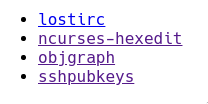
\includegraphics[]{../Pictures/overview.png}}
\caption{Overview of rebuild packages}%
\label{fig:rebuild-overview} 
\end{figure}

\begin{figure}[H]
\center{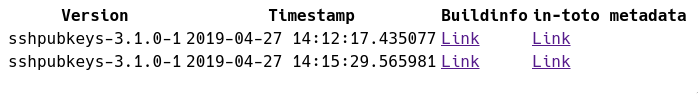
\includegraphics[width=\textwidth]{../Pictures/sources-view.png}}
\caption{Overview of the rebuild submissions}%
\label{fig:submission-overview} 
\end{figure}

The website as shown on Figure~\ref{fig:rebuild-overview} and
Figure~\ref{fig:submission-overview} displays the finished webserver for the
initial rewrite of the visualizer. The resulting code and webpage maintains
compatibility of the existing visualizer and enables us to continue implementing
further improvements on the API.

\subsection{Second Iteration: Merkle Tree}%
\label{sub:merkle_tree}
The second iteration focuses on implementing merkle trees into the visualizer.
These will create the foundation of the transparency log in the upcoming
iterations for this project.

These will be implemented along side of the reimplementation of the visualizer,
and the current structure of the code. We will take a look at the challenges of
implementing this correctly along with making sure the proofs are correctly
implemented to support a transparency log.

\subsection*{Goals}%
\label{sub:second_iteration_goals}
The goals of this iteration is as to make sure the merkle tree operated
properly. For this to happen there needs to be validated proofs and a proper
tree generated when new items are added.

\begin{itemize}
    \item Implement the needed database models for the datastructure
    \item New items should be appended to the tree
    \item The tree should not be rebuilt for each append
    \item Audit proofs should be implemented
    \item Consistency proofs should be implemented
    \item Graph the tree
\end{itemize}


\subsection*{Development}%
\label{sub:second_iteration_development}
The main challenge in this iteration is getting the underlying data model
correct. What we are trying to achieve is to implement a tree structure where
the hash of the leafs is hashed together to form a chain of checksums all the
way up to the tree root. The following algorithm to achieve this is described
below.

The development of this project will be done in a few stages. First we will take
a look at the underlying database model needed to construct the trees. Next up
is how to construct merkel trees without rebuilding all interior nodes. We need
to have a way to append new nodes by rehashing the least amount of interior
hashes.

The next development challenge in this iteration is to make sure the proofs are
working. Without appropriate proofs, mainly audit proofs and consistency proofs
as described in subsection~\ref{sub:certificate_transparency_log}. We will go
through the development of these features and make sure they are working before
moving on for the next iteration.


\subsection*{Database}%
\label{sub:database}
Since we have implemented the visualizer with ``sqlalchemy'', the idea is to
utilize the SQL backend to store the tree. This gives a few challenges on how to
structure the model when it comes with relationships. We need to traverse the
tree for the proofs developed later on, so there should be easy rely on and
construct when constructing new nodes.

\begin{listing}[H]
\begin{minted}[linenos,numbersep=5pt,frame=lines,framesep=2mm]{python}
class Node(db.Model):
    __tablename__ = "node"
    id = db.Column(
        db.Integer(), index=True, unique=True, primary_key=True, autoincrement=True
    )
    leaf_index = db.Column(db.Integer(), default=0)
    type = db.Column(db.String(10), nullable=False)
    hash = db.Column(db.String(128))
    created = db.Column(db.DateTime, nullable=False, default=datetime.utcnow)
    data = db.Column(JSONB)
    height = db.Column(db.Integer(), default=0)
    children_right_id = db.Column(db.Integer, db.ForeignKey("node.id"))
    children_left_id = db.Column(db.Integer, db.ForeignKey("node.id"))

    right = db.relationship("Node",
            foreign_keys='Node.children_right_id',
            uselist=False,
            backref=db.backref('children_right', remote_side=[id]))

    left = db.relationship("Node", 
            foreign_keys='Node.children_left_id',
            uselist=False,
            backref=db.backref('children_left', remote_side=[id]))

    children_id = db.Column(db.Integer, db.ForeignKey("node.id"))
\end{minted}
\caption{Node sqlalchemy model}
\label{lst:node_model}
\end{listing}

Listing~\ref{lst:node_model} shows the model that was settled on. Each of the
fields serve a purpose in the current model. ``leaf\_index'' keeps track of what
position as leaf node it is. This is important when we start constructing proofs
as some of the lookups needs to know what leaf number 16 is. ``type'' denotes
one of two things, ``data'' for leaf nodes or ``level'' for interior nodes.
``data'' is a leaf node that has the ``data'' field filled with JSON. ``level''
has no ``data'' field, but does have both ``left'' and ``right'' filled with the
appropriate child node. ``hash'' contains the hash of the ``data'' JSON object.

The relationship modeled was a bit difficult to get correctly modeled in SQL.
The intentions was to have one foreign key to bind the left and right
relationships to, but this turned out to be difficult to implement. The solution
was to have the ``left'' relationship bind to ``children\_left\_id'' and
``right'' bind to ``children\_right\_id''. This solves the problem of having the
relationship correctly modeled, however to find the correct child node for the
leaf and interior node, we need to check both left and right to find the correct
node.

\begin{figure}[hbst]
\centering
\begin{tikzpicture}
\Tree
[ .r
[ .n1   [ .l ]  [ .r ]  ]
[ .n2 ]
]
\end{tikzpicture}
\caption{Example for relationships}
\label{fig:relationship_example}
\end{figure}

In the example node relationship in Figure~\ref{fig:relationship_example} we can
demonstrate what the ORM described in Listing~\ref{lst:node_model} would end up
looking like. If we sit with the appropriate model for ``N1'' we have a interior
node with a parent, left and right relationship. The parent node ``r'' where
we can peak at the values ``children\_left'' and ``children\_right'' values to
find the correct node. To find the ``l'' and ``r'' leaf nodes in this example we
only have to check the ``left'' and ``right'' relationships respectively.

We are keeping everything in the same table with the same model. There is no
inherent distinction between leafs, interior nodes and root nodes in this
implementation when it comes to the model except for what is specified in the
``types'' direction. To find the root node in this implementation we only have
to look for the last inserted ``level'' node.

\subsection*{Construct tree}%
\label{sub:construct_tree}
We now have the database model we can build the tree with. Since this system is
suppose to run over time, and might target thousands of nodes, we need to be
able to append to the tree without re building the entire tree. This is a
tedious process and could very well take quite a while if the number of nodes
grow large enough.

The algorithm to build a tree, where all the interior nodes are hashed for every
new insertion involves counting the number of nodes to be hashed. If this is an
odd number, promote the last node in this list to the next step. Now we take two
and two nodes and hash them together, left to right. This creates interior nodes
we call ``levels''. When this is done, we start from the beginning and the
current set of interior nodes are the nodes we operate on.

This is a tedious process and does not scale very well over time. What we do
need is an algorithm that only rehash the changed interior nodes.

The algorithm for this involves figuring out all the loose subroots of the tree.
This approach to append new notes has been described in the original paper
by~\citeauthor{182788} where they calculate frozen subroots down on the left
Side of the tree until the appropriate subroot is reached~\cite{182788}.

Our implementation is as follows; we take the count of all leafs in the tree and
use them to calculate the largest complete subtree in the merkle tree, and
remove this from the count.  What we are left with are all the nodes in surplus
on the right hand side of the tree.

We can then walk down the tree on the left side, append the current node on the
path, and then do the same calculation with the nodes in surplus. We then know
the next complete subtree in the chain, remove them from the count, append the
node and walk down. We continue this until we reach 0 loose nodes, in which case
we are at the node we are suppose to append the new node with. The chain of
appended nodes upwards is the list of nodes we need to append with to rehash all
of the interior nodes of the tree.

The resulting code takes the new node that is going to be appended and hashes it
in the with the lowest node going up. This only rehashes the interior nodes of
the tree that needs to be rehashed. This lets us very easily reach a fast
append-only merkel-tree implementation backed by a SQL database.


\subsection*{Cryptographic attack mitigation}%
\label{sub:mitigate_attack}
To the nodes we need to consider the two sources of information we are
essentially hashing. If the node is a leaf we need to hash the JSON data
structure. This is done by taking the keys and values in the JSON structure and
hashing them together in order. If the node is a interior node, this step is
omitted and the hash consists of the hash of the left and right nodes as shown
in Listing~\ref{lst:node_hashing_strategy}. The result of this is the
appropriate hash for the node.

\begin{listing}[H]
\caption{Node hashing strategy}
\label{lst:node_hashing_strategy}
\begin{equation*}
H\{\text{NodeType},\ \text{LeftNode},\ \text{RightNode}\}
\end{equation*}
\end{listing}

There are a few attacks on can do in practice on any data structure that uses
cryptographic hashes. Since the same output always returns the same value, they
are prone to what is called a ``second preimage'' attack~\cite{rfc4270}. If the
attacker know the input, they can re append the values, and create the same hash
in the tree.  This can allow the construction of malicious data or open up for
other venues of attack.

To mitigate this, certificate transparency log append a null byte value for
leafs, and a 1 byte value for levels in the tree. This makes sure that we can't
replay previous data as there is always some values being appended. In our
implementation we append ``data'' and ``level'' as the prefix in the hashed
value. This serves the same purpose as the certificate transparency logs.


\subsection*{Graphviz}%
\label{sub:graph_merkle_tree}
To validate that we are getting the correct association and relationships when
appending new elements, one of the important things to get is a visualization of
the currently constructed merkle tree. To aid the discovery of problematic nodes
the first 10 letters of the hash is printed with the node to easily find the
affected node and aid debugging.

To do this we loop through all of the nodes in the tree. We print out the left,
and right parent of the node in a format that is compatible with the graphviz
tool to generate pictures. The output found in Listing~\ref{lst:graphviz-test}
enables us to produce the PDF picture in Figure~\ref{fig:graphviz_pdf} by
supplying the output to ``dot -Tpdf''.

It should be noted that when trees get sufficiently large, the graph it self is
of less value when debugging. It is hard to get a good overview when the tree
reaches around 60 nodes as the generated trees are spacious. Not enough time was
invested trying to fiddle with the style got a proper display when the trees
grow large enough. However, they did aid in early debugging when trees where
sparse.

\begin{listing}[H]
\caption{Example graph of a generated tree}
\label{lst:graphviz-test}
\begin{minted}{bash}
$ curl 127.0.0.1:5000/api/log/tree/graphviz                        
graph graphname {
labelloc="t";
label="Nodes: 4";
"9A565DAB05" -- "B439C9F4B0";
"9A565DAB05" -- "730212F389";
"B439C9F4B0" -- "47A2AB3D2E";
"B439C9F4B0" -- "648D1817A3";
"730212F389" -- "92EF30AD83";
"730212F389" -- "1E94F9FDE4";
}
\end{minted}
\end{listing}

\begin{figure}[H]
\centering
\includegraphics[width=\textwidth]{../Diagrams/graph.pdf}
\caption{Graphviz visualization}
\label{fig:graphviz_pdf}
\end{figure}


\subsection*{Audit proof}%
\label{sub:audit_proof_implementation}
Audits proofs are important as they prove whether or not a given leaf is part of
the tree. They are used to validate that the data on the leaf is actually part
of a merkle tree. The implementation of this is fairly straight forward as we
have implemented the database structure in a succinct manner.

The audit proof needs the id, or the hash of the node that should have the audit
proof generated. When we have the node, we essentially traverse the children of
the node. We then check on what side of the child the parent node is on. If it's
on the left side, we fetch the right node on the next children. This node is
appended to the list with the keyword ``RIGHT''. If it's on the right side, we
fetch the left node on the next children side. This node is appended to the list
with the keyword ``LEFT''. We then traverse to the next child and continue the
path upwards until the root node is reached, which has no child node.

When all the nodes are appended to a list, with the correct side expressed we
have a complete list of all the nodes needed. We can then append the current
root node to the response and let users hash the path and recreate the current
root node.

The appropriate JSON response for an example tree can be found in
Listing~\ref{lst:audit proof}. For the sake of being terse, some auxiliary
fields have been omitted in this example. In this case, to recreate the root
found in the top of the JSON output, we would just have to hash the ``path'' as
given and append the hash on the correct side of the previous hash.

\begin{listing}[htpb]
\caption{JSON for audit proof}
\label{lst:audit proof}
\begin{minted}{json}
$ curl 127.0.0.1:5000/api/log/tree/validate/id/1
{"root": {
    "id": 8,
    "type": "level",
    "hash": "9a565dab05",
    "right": "730212f389",
    "left": "b439c9f4b0" },
  "path": [
      ["LEFT", {
        "id": 1,
        "type": "data",
        "hash": "47a2ab3d2e",
        "parent": "b439c9f4b0",
        "data": { ... }}],
    ["RIGHT", {
        "id": 2,
        "type": "data",
        "hash": "648d1817a3",
        "parent": "b439c9f4b0",
        "data": { ... }}],
    ["RIGHT", {
        "id": 7,
        "type": "level",
        "hash": "730212f389",
        "right": "1e94f9fde4",
        "left": "92ef30ad83",
        "parent": "9a565dab05"}]],
  "validation": true}
\end{minted}
\end{listing}


\subsection*{Consistency proof}%
\label{sub:consistency_proof_implementation}


\begin{listing}[H]
\caption{JSON for consistency proof}
\label{lst:consistency proof}
\begin{minted}{json}
{"root": {
    "id": 8,
    "type": "level",
    "hash": "9a565dab05",
    "right": "730212f389",
    "left": "b439c9f4b0"},
  "path": [
      ["LEFT", {
        "id": 3,
        "type": "level",
        "hash": "b439c9f4b0",
        "right": "648d1817a3",
        "left": "47a2ab3d2e",
        "parent": "9a565dab05"}],
      ["RIGHT", {
        "id": 7,
        "type": "level",
        "hash": "730212f389",
        "right": "1e94f9fde4",
        "left": "92ef30ad83",
        "parent": "9a565dab05",
        "data": {}}]],
  "inclusion": true,
  "consistency": true}
\end{minted}
\end{listing}

\subsection*{Results}%
\label{sub:second_iteration_results}


\begin{table}[H]
\footnotesize
\centering
\settowidth\tymin{\textbf{Description}}
\setlength\extrarowheight{2pt}
\begin{tabulary}{1.0\textwidth}{|l|L|l|L|}
\hline
    \textbf{Endpoint} & 
    \textbf{Type} & 
    \textbf{Parameters} & 
    \textbf{Description} \\
\hline
    /api/log/stats & GET & & Statistics from the current tree \\ \hline
    /api/log/graphviz & GET & & Outputs the current tree in the dot format \\ \hline
    /api/log/root & GET & & Gets the latest tree root \\ \hline
    /api/log/tree/append & POST & JSON object & Appends a JSON object to the tree \\ \hline
    /api/log/tree/id/<id> & GET & & Gets the given Node object from the database with '``id''\\ \hline
    /api/log/tree/hash/<hash> & GET & & Gets the given Node object from the database with ``hash''\\ \hline
    /api/log/tree/leaf/<id> & GET & & Gets the given leaf from the database with matching ``leaf\_index''\\ \hline
    /api/log/tree/validate/id/<id> & GET & & Gets the audit proof for a leaf matching the given ``id''\\ \hline
    /api/log/tree/validate/hash/<hash> & GET & & Gets the audit proof for a leaf matching the given ``hash''\\ \hline
    %/api/log/tree/inclusion & POST & InclusionQuery & Provides the inclusion proof for the given query \\ \hline
    /api/log/tree/consistency & POST & ConsistencyQuery & Provides the consistency proof for the given query\\ \hline
\end{tabulary}
\caption{Second iteration: Transparency log API}
\label{api:transparency_log}
\end{table}



\subsection{Third Iteration: Tree root signing}%
\label{sub:tree_root_signing}
One essential part of merkle trees as implemented
by~\citeauthor{b.-laurie-a.-langley-e.kaster-google-2013} in certificate
transparency logs is the ability to have tree-roots
signed~\cite{b.-laurie-a.-langley-e.kaster-google-2013}. This lets us verify
with public key cryptography that the tree-root was created by the given
transparency log. In this chapter we will go through how this implemented.

\subsection*{Goals}%
\label{sub:third_iteration_goals}

The goals of this iteration is to create the needed code to create and verify
signatures on tree nodes.

\begin{itemize}
    \item Initialize signing keys
    \item Sign every tree root created by the log
    \item Verify the signature
\end{itemize}

\subsection*{Development}%
\label{sub:third_iteration_development}
For the development of this feature we are utilizing the ``securesystemslib'' from
New York University's' secure systems lab. It's a library with a collection of
easy-to-use primitives to deal with encryption, decryption and signature
verification on data for python. Utilizing this library makes it trivial to
implement the needed signature functionality in a short concise manner.

\begin{listing}[H]
\caption{Glue code for ``securesystemslib''}
\label{lst:securesystemslib_glue}
\begin{minted}[linenos,numbersep=5pt,frame=lines,framesep=2mm]{python}
PASSWORD = "123"
KEY_NAME = "ed25519_key"

def init_keys():
    if not os.path.isfile(KEY_NAME):
        generate_and_write_ed25519_keypair(KEY_NAME, password=PASSWORD)

def get_private_key():
    init_keys()
    return import_ed25519_privatekey_from_file(KEY_NAME, password=PASSWORD)

def get_public_key():
    init_keys()
    return import_ed25519_publickey_from_file(KEY_NAME+'.pub')

def sign_data(data):
    return create_signature(get_private_key(), data)

def verify_data(signature, data):
    return verify_signature(get_private_key(), signature, data)
\end{minted}
\end{listing}

The implementation itself consists of a file for the needed code to ease the key
creation for the rebuilder. For the sake of ease, we don't consider problems
such as password strength for the signing key as the main focus is on the
transparency log implementation, so in this implementation the password is
hard coded to ``123'', which is admittedly a poor password. For the
cryptography, elliptic curves are used instead of the traditional RSA algorithm.
The choice behind this is because elliptic curves needs less bits to produce
equally strong keys. We then end up with faster and smaller signatures.

These auxiliary functions makes it trivial to further implement the tree root
signing in the model.

\begin{listing}[H]
\caption{Additions to the Node model}
\label{lst:node_tree_root_signature}
\begin{minted}{diff}
@@ -21,10 +22,10 @@ class Node(db.Model):
     leaf_index = db.Column(db.Integer(), default=0)
     type = db.Column(db.String(10), nullable=False)
     hash = db.Column(db.String(128))
+    signature = db.Column(db.String(128))
     created = db.Column(db.DateTime, nullable=False, default=datetime.utcnow)
     data = db.Column(JSONB)
     height = db.Column(db.Integer(), default=0)
\end{minted}
\end{listing}

In Listing~\ref{lst:node_tree_root_signature} we can see the additions to the
``Node'' model from Listing~\ref{lst:node_model} page~\pageref{lst:node_model}.
This enables us to store the signature string in the database model for future
use when creating tree roots.

\begin{listing}[H]
\caption{Additions to the append function}
\label{lst:append_tree_root_signing}
\begin{minted}{diff}
@@ -166,7 +168,9 @@ def append(data):
     for node in reversed(subtrees):
         new_parent = create_level_node(node, new_node)
         new_node = new_parent
+    signature = sign_data(new_node.hash)
+    new_node.signature = signature["sig"]
     db.session.commit()
     return ret
\end{minted}
\end{listing}

Listing~\ref{lst:append_tree_root_signing} shows the additions made to the
``append'' function to support signed tree roots. Since the last ``new\_node'' is
the new tree root, we only sign the hash of this node. This is enough to
implement tree root signing in the current implementation of the visualizer.

\subsection*{Results}%
\label{sub:third_iteration_results}

The results of this iteration is 2 new endpoints and some new code to help with
signing tree roots in the transparency log. The resulting API endpoints can be
found in Table~\ref{api:crypto_api} which shows the newly created endpoints.

\begin{table}[H]
\footnotesize
\centering
\settowidth\tymin{\textbf{Description}}
\setlength\extrarowheight{2pt}
\begin{tabulary}{1.0\textwidth}{|l|L|l|L|}
\hline
    \textbf{Endpoint} & 
    \textbf{Type} & 
    \textbf{Parameters} & 
    \textbf{Description} \\
\hline
    /api/crypto/key & GET & & Outputs the key object used by the library \\ \hline
    /api/crypto/validate & POST & Tree root & Validates the tree root to the public key \\ \hline
\end{tabulary}
\caption{Third Iteration: Crypto API }
\label{api:crypto_api}
\end{table}

The usage of the endpoints is fairly straight forward. We can call the generated
signing key with ``/api/crypto/key'' as shown
in~\ref{lst:display-generated-public-key}. Which enables us to verify the
signature on the client side instead of on the server side if we need to do
that.

\begin{listing}[H]
\caption{Display generated public key}
\label{lst:display-generated-public-key}
\begin{minted}{bash}
$ curl 127.0.0.1:5000/api/key
{
  "keytype": "ed25519",
  "scheme": "ed25519",
  "keyid": "25a16bb3a3...",
  "keyid_hash_algorithms": [
    "sha256",
    "sha512"
  ],
  "keyval": {
    "public": "7623ba359c..."
  }
}
\end{minted}
\end{listing}

To verify a tree root on the server side, we can provide the output from
``/api/log/tree/root'' from Listing~\ref{api:transparency_log}, and forward this
to ``/api/crypto/verify''. In the example from
Listing~\ref{lst:test-verify-endpoint}, we have provided a minimal tree root
json object to display a successful verification of a tree root on the server
side.

\begin{listing}[H]
\caption{Test of the verify endpoint}
\label{lst:test-verify-endpoint}
\begin{minted}{bash}
$ curl --header "Content-Type: application/json" \
  --request POST \
  --data '{"hash": "21e0b13a6f...", \
           "signature": "832510c0188..."}' \
  127.0.0.1:5000/api/crypto/verify
{
  "status": "ok",
  "verified": true
}
\end{minted}
\end{listing}


\subsection{Fourth Iteration: Transparency log overlay}%
\label{sub:transparency_overlay}

\subsection*{Goals}%
\label{sub:fourth_iteration_goals}

\subsection*{Development}%
\label{sub:fourth_iteration_development}

API entry definitions

\begin{listing}[H]
\caption{Entry definitions}
\label{lst:entrydefinitions}
\begin{minted}[linenos,numbersep=5pt,frame=lines,framesep=2mm]{go}
type Entry {
    Package string
    Version string
} 

type InclusionEntry {
    Entry
    Buildinfo       string
    Linkmetadata    string
}

type RevokeEntry {
    Entry 
    InclusionHash   string
    Reason          string
}
\end{minted}
\end{listing}


\begin{table}[hbtp]
\footnotesize
\centering
\settowidth\tymin{\textbf{Description}}
\setlength\extrarowheight{2pt}
\begin{tabulary}{1.0\textwidth}{|l|L|L|L|}
\hline
    \textbf{Endpoint} & 
    \textbf{Type} & 
    \textbf{Parameters} & 
    \textbf{Description} \\
\hline
    /api/rebuilder/submit & POST$^1$ & metadata, buildinfo& Implements something heyho lets go \\  \hline
    /api/rebuilder/revoke& POST$^1$ & leaf hash, reason, signature& Revokes the leaf with a reason  \\  \hline
    /api/rebuilder/fetch/<name>/<version>& GET & & Gets the entries for the given package \\  \hline
\end{tabulary}
\footnotesize{$^1$ Behind authentication}\\
\caption{Overlay API}
\label{api:Overlay API}
\end{table}

\subsection*{Results}%
\label{sub:fourth_iteration_results}


\subsection{APT Transport integration}\label{sec:apt_transport}

\begin{figure}[H]
  \centering
  \begin{sequencediagram}
    \newthread{A}{HTTP client}{}
    \newinst[1]{B}{intoto}{}
    \newinst[2]{C}{APT Server}{}
    \begin{messcall}{A}{100 Capabilities}{C}
        \begin{messcall}{C}{601 Configuration}{A}\end{messcall}
        \begin{messcall}{C}{600 URI Acquire}{A}\end{messcall}
        \begin{messcall}{A}{200 URI Start}{C}\end{messcall}
            \begin{messcall}{C}{201 URI Done}{B}
                \begin{sdblock}{Rebuilder verify}{}
                    \begin{messcall}{B}{201 URI Done}{A}\end{messcall}
                \end{sdblock}
            \end{messcall}
    \end{messcall}
  \end{sequencediagram}
\caption{intoto sequence diagram}
\label{lst:intoto_sequence_diagram}
\end{figure}

\begin{listing}[H]
\caption{Initial API request}
\label{lst:init_request}
\begin{align*}
& \text{InitQuery}\{\text{Hash},\ \text{Signature},\ \text{LeafCount}\} \to \\
& \text{Response}\{\text{ConsistencyProof},\ \text{CurrentRoot}\{\text{Hash},\ \text{Signature}\} \}
\end{align*}
\end{listing}


\begin{listing}[H]
\caption{Package query API request}
\label{lst:package_query_request}
\begin{equation*}
    \text{PkgQuery}\{\text{Package},\ \text{Version}\} \to \text{Response}\{\text{InclusionEntry},\ \text{Entry}\dots \}
\end{equation*}
\end{listing}


\section{Testing}%
\label{sec:testing}


\blankpage
\end{document}
